\documentclass{llncs}  

\usepackage{url}
\usepackage[noend]{algorithm2e}
\usepackage{amsmath}
\usepackage{amssymb}
\usepackage{etoolbox}
\usepackage{multirow}     
\usepackage[usenames,dvipsnames]{color}
\usepackage{tikz}
\usetikzlibrary{arrows,calc}
\usepackage{caption}
\usepackage{subcaption}
\usepackage{varwidth}
\captionsetup{compatibility=false}
\usepackage{listings}
\lstset{
  morekeywords={define,end,if,then,else,return,assume,assert},
  basicstyle=\ttfamily,
  keywordstyle=\underline,
  numbers=left,
  frame=l
}
\usepackage{bussproofs}

\newcommand{\smallnode}[1]{\begin{varwidth}{0.4cm}\scalebox{0.9}{\hspace{-0.2cm}#1}\end{varwidth}}
\newcommand{\todo}[1]{\textcolor{red}{{#1}}}
\newcommand{\hide}[1]{}
\newcommand{\fun}[1]{\mathtt{{#1}}}
\newcommand{\TT}{\mathtt{true}}
\newcommand{\FF}{\mathtt{false}}

 
%\newcommand{\longversion}{}
\ifdef{\longversion}{
\newcommand{\whenlongversion}[1]{#1}
}{
\newcommand{\whenlongversion}[1]{}
}

\newcommand{\ox}{\textbf{x}}
\newcommand{\ou}{\textbf{u}}
\newcommand{\ov}{\textbf{v}}
\newcommand{\oE}{\textbf{E}}
\newcommand{\assert}[1]{(\!| {#1} |\!)}

\title{Verifying Recursive Programs using Intraprocedural 
Analyzers}
\author{Yu-Fang~Chen\inst{1} \and Chiao~Hsieh\inst{1,2} \and 
  Ming-Hsien~Tsai\inst{1} \and Bow-Yaw~Wang\inst{1} \and Farn~Wang\inst{2}}

\institute{
Institute of Information Science, 
Academia Sinica, Taiwan
\and
Graduate Institute of Electrical Engineering,
National Taiwan University, Taiwan
}

\pagestyle{plain}
\sloppy

\begin{document}
\maketitle

\begin{abstract}

Recursion can complicate program analysis significantly. 
Some program analyzers simply ignore recursion or even refuse
to check 
recursive programs. In this paper, we propose an algorithm that uses
a recursion-free program analyzer as a black box to check recursive
programs. With extended program constructs for assumptions,
assertions, and nondeterministic values, our algorithm computes
function summaries from inductive invariants computed by the
underlying program analyzer. Such function summaries enable our
algorithm to check recursive programs. We implement a prototype using
the recursion-free program analyzer \textsc{CPAChecker} and compare it
with other program analyzers on the benchmarks in the 2014 Competition
on Software Verification.

\end{abstract}

\section{Introduction}
\label{section:introduction}

Program verification is a grand challenge in computer science with significant practical impact. 
The difficulty of this problem due in great part to several complex common constructs of conventional programming languages~\cite{ClarkeJS05}, e.g., concurrent execution of threads, pointers with unbounded heap size, function call with recursions, and unbounded/large basic data types. It is unlikely to develop a verification algorithm that handles all of these constructs. Very commonly, researches on program verification focus on only a few of these constructs and have simplified assumptions on the rest. Moreover, the verification tools become more and more unmanageable with the increased number of constructs they support. Updating the existing verification tools to include new solutions dealing with more program constructs is normally a nightmare for the developers.

In the paper, we propose a loosely-coupled approach to enable existing intraprocedure analyzers the capability of handling recursive functions. 




\section{Preliminaries}
\label{section:preliminaries}


Let $\mathtt{Vars}$ denote the set of \emph{program variables} and
$\mathtt{Vars}' = \{ \ox' : \ox \in \mathtt{Vars} \}$.
We consider a variant of the WHILE language~\cite{}:
\begin{equation*}
  \begin{array}{rccll}
    \mathtt{Expression} & \ni E & ::= &
    \mathtt{x} & \mathtt{x} \in \mathtt{Vars}\\
    & & \mid &
    \mathtt{false}\ \mid\ \mathtt{true}\ \mid\ 
    \mathtt{0}\ \mid\ \mathtt{1}\ \mid\ \ldots\hspace{.06\textwidth} &
    \textmd{constant}\\
    & & \mid &
    E \odot E  & \odot \in \{ +, -, =, >, \mathtt{and} \}\\
    & & \mid & \mathtt{not}\ E\\
    & & \mid &
    \mathtt{f}(E, E, \ldots, E) &
    \textmd{function invocation}\\
    \mathtt{Command} & \ni C & ::= &
    \mathtt{x}, \mathtt{x}, \ldots, \mathtt{x} := 
    E, E, \ldots, E & \textmd{assignment}\\
    & & \mid &
    \mathtt{assume}\ E & \textmd{assumption}\\
    & & \mid &
    \mathtt{assert}\ E & \textmd{assertion}\\
    & & \mid &
    \mathtt{return}\ E, E, \ldots, E & \textmd{function return}\\
  \end{array}
\end{equation*}
Note that simultaneous assignments are allowed in our language. To
execute a simultaneous assignment, all expressions on the right hand
side are first evaluated and then assign to respective variables. The
assumption command excludes all computation not satisfying the given
expression. The assert command terminates computation
abnormally if the given expression is not satisfied. For
instance, the following command always terminates normally:
\begin{equation*}
  \mathtt{assume\ false};\ \ \mathtt{assert\ false}
\end{equation*}
\todo{no computation means terminate normally?}
Our simple language also allows functions to return multiple
values. Together with simultaneous assignments, functions can update
several variables at once.

A function is represented as a \emph{control flow graph} $G = \langle
V, E \rangle$ where the nodes in $V$ are \emph{program locations}, and
each edge $(\ell, \ell')$ in $E \subseteq V \times V$ is labeled by a
command denoted by $\textmd{cmd} (\ell, \ell')$. We
assume that the program locations $\ell_s$ and $\ell_e$ denote the
entry and exit of each function. Moreover, the special
$\mathtt{main()}$ function specifies where a program starts.
Figure~\ref{figure:mccarthy91} shows control flow graphs for the
McCarthy 91 program. The $\mathtt{main()}$ function assumes the
variable $\mathtt{n}$ is non-negative. It then checks
$\mathtt{mc91(n)}$ is no less than 90
(Figure~\ref{figure:mccarthy91:main}). The $\mathtt{mc91(n)}$ function
branches on whether the variable $\mathtt{n}$ is greater than 100. If
so, $\mathtt{mc91(n)}$ returns $\mathtt{n} - 10$. Otherwise,
$\mathtt{mc91(n)}$ returns $\mathtt{mc91(mc91(n + 11))}$
(Figure~\ref{figure:mccarthy91:mc91}). Observe that the
$\mathtt{assume}$ command models a conditional branch in the
figure. Loops can be modeled similarly.

\begin{figure}
  \centering
  \begin{subfigure}[b]{.3\textwidth}
    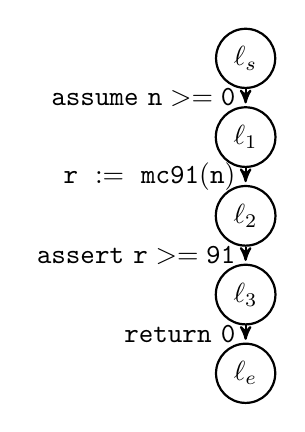
\begin{tikzpicture}[->,>=stealth',shorten >=1pt,auto,node
      distance=2cm,thick,node/.style={circle,draw}]
      \node[node] (0) at (0, 0) {$\ell_s$}; %[label=above:$\mathtt{main()}$]
      \node[node] (1) at (0, -1) {$\ell_1$};
      \node[node] (2) at (0, -2) {$\ell_2$};
      \node[node] (3) at (0, -3) {$\ell_3$};
      \node[node] (4) at (0, -4) {$\ell_e$};

      \path
        (0) edge 
            node [left] {$\mathtt{assume\ n >= 0}$} (1)
        (1) edge 
            node [left] {$\mathtt{r\ :=\ mc91(n)}$} (2)
        (2) edge 
            node [left] {$\mathtt{assert\ r >= 91}$} (3)
        (3) edge 
            node [left] {$\mathtt{return\ 0}$} (4);
    \end{tikzpicture}
    \caption{$\mathtt{main()}$}
    \label{figure:mccarthy91:main}
  \end{subfigure}
  ~
  \begin{subfigure}[b]{.6\textwidth}
    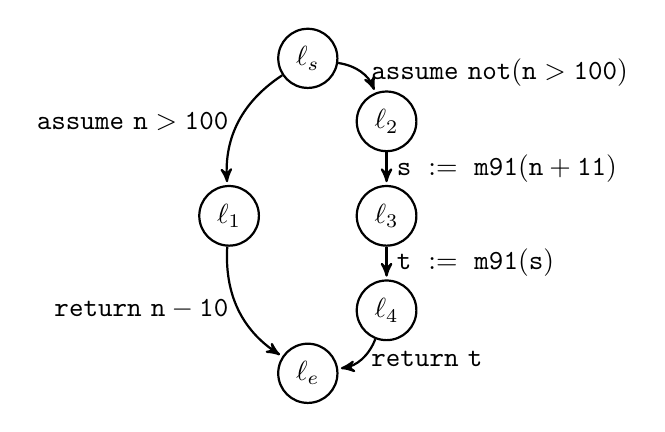
\begin{tikzpicture}[->,>=stealth',shorten >=1pt,auto,node
      distance=2cm,thick,node/.style={circle,draw}]
      \node[node] (0) at ( 0,  0) {$\ell_s$}; %[label=above:$\mathtt{mc91(n)}$]
      \node[node] (1) at (-1, -2) {$\ell_1$};
      \node[node] (2) at ( 1, -0.8) {$\ell_2$};
      \node[node] (3) at ( 1, -2) {$\ell_3$};
      \node[node] (4) at ( 1, -3.2) {$\ell_4$};
      \node[node] (5) at ( 0, -4) {$\ell_e$};

      \path
        (0) edge [bend right=30]
            node [left] {$\mathtt{assume\ n > 100}$} (1)
            edge [bend left=30]
            node [right] {$\mathtt{assume\ not(n > 100)}$} (2)
        (1) edge [bend right=30]
            node [left] {$\mathtt{return\ n - 10}$} (5)
        (2) edge 
            node [right] {$\mathtt{s\ :=\ m91(n + 11)}$} (3)
        (3) edge 
            node [right] {$\mathtt{t\ :=\ m91(s)}$} (4)
        (4) edge [bend left=30]
            node [right] {$\mathtt{return\ t}$} (5);
    \end{tikzpicture}
    \caption{$\mathtt{mc91(n)}$}
    \label{figure:mccarthy91:mc91}
  \end{subfigure}
  \caption{McCarthy 91}
  \label{figure:mccarthy91}
\end{figure}

\todo{definitions of accessible variables, program states}
Let $G = \langle V, E \rangle$ be a control flow graph.
An \emph{inductive invariant} $\Pi (G, I_0) = \{ I_\ell : \ell \in V
\}$ for $G$ from $I_0$ is a set of first-order logic formulae such
that $I_{\ell_s} = I_0$, and for every $(\ell, \ell') \in E$
\begin{equation*}
I_{\ell} \wedge \tau_{\textmd{cmd}(\ell, \ell')} \implies I'_{\ell'}
\end{equation*}
where $I'$ is the formula obtained by replacing every $\ox \in
\mathtt{Vars}$ in $I$ with $\ox' \in \mathtt{Vars}'$, and
$\tau_{\textmd{cmd} (e)}$ specifies the semantics of the command
$\textmd{cmd} (e)$. An inductive invariant $\Pi (G, I_0)$ is an
over-approximation to the computation of $G$ from $I_0$. More
precisely, assume that the function $G$ starts from a state satisfying
$I_0$. For every program location $\ell$, $G$ must arrive in a state
satisfying $I_{\ell}$ when the computation reaches $\ell$. Observe
that an inductive invariant $\Pi (G, I_0)$ establishes the weak
correctness for the Hoare triple $\{ I_0 \} G \{ I_{\ell_e} \}$.

A \emph{program analyzer} accepts programs as inputs and
checks if all assertions (specified by the $\mathtt{assert}$ command)
are satisfied. One way to implement program analyzers is to compute
inductive invariants. 
\begin{proposition}
Let $G = \langle V, E \rangle$ be a control flow
graph and $\Pi (G, \mathtt{true})$ an inductive invariant for $G$ from
$\mathtt{true}$. If $\models I_{\ell} \implies B_{\ell}$ for every
edge $(\ell, \ell') \in E$ with $\textmd{cmd} (\ell, \ell') =
\mathtt{assert} (B_{\ell})$, then all assertions in $G$ are satisfied.
\end{proposition}
A program analyzer checks assertions by computing inductive invariants
is called an \emph{inductive} program analyzer. Note that an inductive
program analyzer need not give any information when an assertion fails. 
Indeed, most inductive program analyzers simply report false positives
when inductive invariants are too coarse. A \emph{program checker} is
a program analyzer that returns an error trace when an assertion
fails; an \emph{error trace} is a sequence of variable valuations from
the program entry to the failed assertion. Rather than reporting false
positives, program checkers have to return error traces to witness 
failed assertions. Producing error traces (especially for recursive
programs) complicates analysis algorithms. We hence consider a
subclass of program checker. A \emph{recursion-free
  inductive program checker} is a program checker that checks
recursion-free programs by computing inductive invariants, and reports
an error trace when an assertion fails. Several recursion-free
inductive program checkers are available such as \textsc{CPAChecker},
\textsc{Blast}, \textsc{SLAM} \todo{more?}. Our goal is to check
recursive programs by using a recursion-free inductive program checker
as a black box. 


\section{Overview}
\label{section:overview}


Let \textsc{BasicChecker} denote a recursion-free inductive program
checker and $G = \langle V, E \rangle$ a control flow graph. Since
non-recursive functions can be replaced by their control flow graphs
after proper variable renaming, we assume that $G$ only contains the
$\mathtt{main()}$ and recursive functions. If $G$ does not contain
recursive functions, \textsc{BasicChecker} is able to check $G$ by
computing inductive invariants.

When $G$ contains recursive functions, we transform $G$ into two
recursion-free programs $\underline{G}$ and $\overline{G}$. The
program $\underline{G}$ under-approximates the computation of
$G$. That is, every computation of $\underline{G}$ is also a
computation of $G$. If \textsc{BasicChecker} finds an error trace in
$\underline{G}$, our algorithm terminates and reports the error
trace. The program $\overline{G}$ on the other hand over-approximates
the computation of $G$; every computation of $G$ is also a computation
of $\overline{G}$. If \textsc{BasicChecker} proves that all assertions
in $\overline{G}$ are satisfied, our algorithm terminates and reports
that all assertions in $G$ are satisfied. If \textsc{BasicChecker}
fails to prove assertions in $\overline{G}$, our algorithm refines the
approximations by unwinding recursive functions and
reiterates~(Algorithm~\ref{algorithm:overview}). 

\begin{algorithm}
  \KwIn{$G = \langle V, E \rangle$ : a control flow graph}
  $k \leftarrow 0$\;
  $G_0 \leftarrow G$\;
  \Repeat{forever}
  {
    \uIf {\textsc{BasicChecker} ($\underline{G}_k$) =
      $\mathit{ErrorTrace} (\tau)$}
    {
      \tcp{find an error trace in the under-approximation $\underline{G}_k$}
      \Return $\mathit{ErrorTrace} (\tau)$\;
    }
    \uElseIf {\textsc{BasicChecker} ($\overline{G}_k$) =
      $\mathit{Pass}$}
    {
      \tcp{prove all assertions in the over-approximation $\overline{G}_k$}
      \Return $\mathit{Pass}$\;
    }
    \uElse {
      $G_{k+1} \leftarrow $ unwind $G_k$\;
      $k \leftarrow k + 1$\;
    }
  }
  \caption{Overview}
  \label{algorithm:overview}
\end{algorithm}

To see how to under approximate computation, consider a control flow
graph $G_k$ with recursive functions $f_0 (\ox_0), f_1 (\ox_1),
\ldots, f_m (\ox_m)$. The under-approximation $\underline{G}_k$ is
obtained by substituting the command $\mathtt{assume\ false}$ for
every command with recursive function calls. The substitution
effectively blocks all recursive invocations. Note that
$\underline{G}_k$ is recursion-free. \textsc{BasicChecker} is able to
check the under-approximation $\underline{G}_k$.

\begin{figure}
  \centering
  \begin{subfigure}[b]{.3\textwidth}
    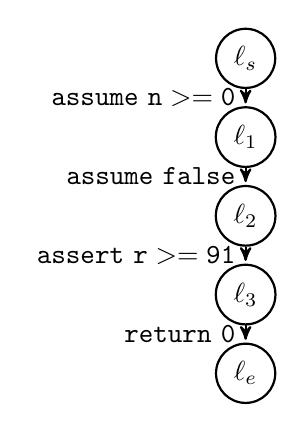
\begin{tikzpicture}[->,>=stealth',shorten >=1pt,auto,node
      distance=2cm,thick,node/.style={circle,draw}]
      \node[node] (0) at (0, 0) {$\ell_s$}; %[label=above:$\mathtt{main()}$]
      \node[node] (1) at (0, -1) {$\ell_1$};
      \node[node] (2) at (0, -2) {$\ell_2$};
      \node[node] (3) at (0, -3) {$\ell_3$};
      \node[node] (4) at (0, -4) {$\ell_e$};

      \path
        (0) edge 
            node [left] {$\mathtt{assume\ n >= 0}$} (1)
        (1) edge 
            node [left] {$\mathtt{assume\ false}$} (2)
        (2) edge 
            node [left] {$\mathtt{assert\ r >= 91}$} (3)
        (3) edge 
            node [left] {$\mathtt{return\ 0}$} (4);
    \end{tikzpicture}
    \caption{$\mathtt{\underline{main}()}$}
  \end{subfigure}
  ~
  \begin{subfigure}[b]{.6\textwidth}
    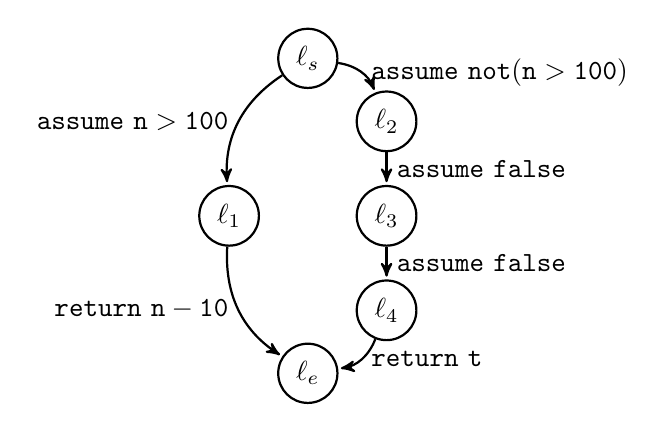
\begin{tikzpicture}[->,>=stealth',shorten >=1pt,auto,node
      distance=2cm,thick,node/.style={circle,draw}]
      \node[node] (0) at ( 0,  0) {$\ell_s$}; %[label=above:$\mathtt{mc91(n)}$]
      \node[node] (1) at (-1, -2) {$\ell_1$};
      \node[node] (2) at ( 1, -0.8) {$\ell_2$};
      \node[node] (3) at ( 1, -2) {$\ell_3$};
      \node[node] (4) at ( 1, -3.2) {$\ell_4$};
      \node[node] (5) at ( 0, -4) {$\ell_e$};

      \path
        (0) edge [bend right=30]
            node [left] {$\mathtt{assume\ n > 100}$} (1)
            edge [bend left=30]
            node [right] {$\mathtt{assume\ not(n > 100)}$} (2)
        (1) edge [bend right=30]
            node [left] {$\mathtt{return\ n - 10}$} (5)
        (2) edge 
            node [right] {$\mathtt{assume\ false}$} (3)
        (3) edge 
            node [right] {$\mathtt{assume\ false}$} (4)
        (4) edge [bend left=30]
            node [right] {$\mathtt{return\ t}$} (5);
    \end{tikzpicture}
    \caption{$\mathtt{\underline{mc91}(n)}$}
  \end{subfigure}
  \caption{Under Approximation of McCarthy 91}
  \label{figure:under-mccarthy91}
\end{figure}



\section{Proving via Transformation}
\label{section:proving-via-transformation}

We give details of the constructions and establish the soundness of
Algorithm~\ref{algorithm:overview}. Throughout this section, we fix an
input control flow graph $G = \langle V, E, \textmd{cmd} \rangle$. For
each function $\mathtt{f}$ in $G$, $G_{\mathtt{f}}$ denotes the
control flow graph of $\mathtt{f}$. Our goal is to establish the
following theorem:

\begin{theorem}
  Let $G = \langle V, E, \textmd{cmd} \rangle$ be a control flow
  graph. If Algorithm~\ref{algorithm:overview} returns
  $\mathit{Pass}$, there is an inductive invariant $\Pi (G, \top)$
  such that $I_{\ell} \implies B_{\ell}$ for every $(\ell, \ell') \in
  E$ with $\textmd{cmd} (\ell, \ell') = \mathtt{assert\ } B_{\ell}$.
  \label{theorem:soundness}
\end{theorem}

By Proposition~\ref{proposition:inductive-invariant}, it follows that
all assertions in $G$ are satisfied.

\subsection{Unwinding}
\label{subsection:unwinding}
Given a CFG $G=\langle
V, E \rangle$. The rename function $\textsc{rename}(G)$ returns a pair of a CFG and a vector of its formal parameters obtained by renaming all variables in $G$ by annotating them with some fresh index numbers. The function $\textsc{unwind}(G)$ (Algorithm~\ref{algorithm:unwind}) returns a CFG obtained by replacing all function call edges in $G$ with the CFG of the called function after renaming. 
\begin{algorithm}
  \KwIn{$G = \langle V, E \rangle$ : a control flow graph}
  $V' \leftarrow V$\;
  $E' \leftarrow E$\;
  \ForEach{$(\ell, \ell')\in E$ with $\textmd{cmd} (\ell, \ell')= x_1,\ldots,x_n:=\mathtt{f}(E_1, \ldots, E_n)$}
  {
  	Let $G_f$ b
  
    \uIf {\textsc{BasicChecker} ($\underline{G}_k$) =
      $\mathit{ErrorTrace} (\tau)$}
    {
      \tcp{find an error trace in the under-approximation $\underline{G}_k$}
      \Return $\mathit{ErrorTrace} (\tau)$\;
    }
    \uElseIf {\textsc{BasicChecker} ($\overline{G}_k$) =
      $\mathit{Pass}$}
    {
      \tcp{prove all assertions in the over-approximation $\overline{G}_k$}
      \Return $\mathit{Pass}$\;
    }
    \uElse {
      $G_{k+1} \leftarrow $ unwind $G_k$\;
      $k \leftarrow k + 1$\;
    }
  }
  \caption{The $\textsc{unwind}(G)$ function}
  \label{algorithm:unwind}
\end{algorithm}


Formally, $\textsc{unwind}(G) = \langle
V', E' \rangle$ such that 
(1) For all edges $(\ell, \ell')\in E$ with $\textmd{cmd} (\ell, \ell')=$

\subsection{Under Approximation}
\label{subsection:under-approximation}

Let $G^\fun{f} = \langle V, E, \textmd{cmd}^\fun{f}, \overline{\texttt{u}}^\fun{f}, \overline{\texttt{r}}^\fun{f},s,e \rangle$ be a control flow
graph. The control flow graph $\underline{G}^\fun{f} = \langle V, E,
\underline{\textmd{cmd}}^\fun{f}, \overline{\texttt{u}}^\fun{f}, \overline{\texttt{r}}^\fun{f},s,e \rangle$ is obtained by replacing every
function calls in $G$ with $\mathtt{assume\ false}$. That is,
\begin{equation*}
  \underline{\textmd{cmd}}^\fun{f} (\ell, \ell') =
  \left\{
    \begin{array}{ll}
      \textmd{cmd}^\fun{f} (\ell, \ell') & 
      \textmd{if } \textmd{cmd}^\fun{f} (\ell, \ell') 
      \textmd{ does not contain function calls}\\
      \mathtt{assume\ false} &
      \textmd{otherwise}
    \end{array}
  \right.
\end{equation*}

\begin{figure}
  \centering
  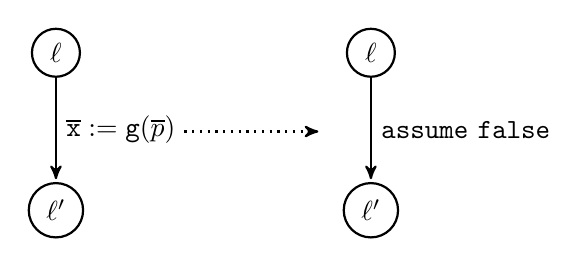
\begin{tikzpicture}[->,>=stealth',shorten >=1pt,auto,node
      distance=2cm,thick,node/.style={circle,draw}]

      \node[node] (0) at (-4, 0)  {$\ell$}; %[label=above:$\mathtt{main()}$]
      \node[node] (1) at (-4, -2) {$\ell'$};

      \node[node] (00) at (0, 0)  {$\ell$};
      \node[node] (01) at (0, -2) {$\ell'$};
      \node (arrow_s) at (-2.5, -1) {};
      \node (arrow_e) at (-0.5, -1) {};

      \path
        (arrow_s) edge [dotted]
                  node {} (arrow_e)
        (0) edge 
            node {$\overline{\mathtt{x}} := \mathtt{g} (\overline{p})$} (1)

        (00) edge 
             node {$\mathtt{assume\ false}$} (01);
    \end{tikzpicture}

  \caption{Under Approximation}
  \label{figure:under-approximation}
\end{figure}

\begin{proposition}
  Let $G^\fun{f}$ be a control flow graph, $P$ and $Q$ logic formulae with
  free variables over program variables of $G$. If $\assert{P}
  G^\fun{f} \assert{Q}$, then 
  $\assert{P} \underline{G}^\fun{f} \assert{Q}$.
\end{proposition}
The above holds because the computations of $\underline{G}^\fun{f}$ under-approximate the computations of $G^\fun{f}$. If all computations of $G^\fun{f}$ from a state satisfying $P$ always end with a state satisfying $Q$, the same should also hold for the computations of $\underline{G}^\fun{f}$.

\subsection{Updating Summary}
\label{subsection:updating-summary}
Let $G^- = \langle V^-, E^-, \textmd{cmd}^- \rangle$ be a CFG obtained from Section~\ref{subsection:under-approximation} and $L_f=\{({\ell_s^i}^{(f)},{\ell_e^i}^{(f)}):\mbox{ the pair of locations }{\ell_s^i}^{(f)}\mbox{ and }{\ell_e^i}^{(f)}\mbox{ in }E\mbox{ for some }i\}$ the set of entry and exit locations of the call to the function $f$.

We give $G^-$ to a program checker. A error trace returned from the checker indicates that some assertion in the program to be verified can be violated, because $G^-$ under-approximates the behavior of $G$. Otherwise, the checker returns an inductive invariant $\Pi (G^-, \mathtt{true})= \{ I_\ell : \ell \in V^-
\}$ for $G^-$. Let $P_f$ be the set of all variables appearing in $G^-$ except the set of formal parameter and return variables of $f$.
Then for all functions $f$ with $L_f\neq \emptyset$, we update the summary of $f$ to $\bigwedge_{(\ell,\ell')\in L_f} \exists P_f. I_\ell \implies \exists P_f.I_{\ell'}$.


\subsection{Checking Summary}
\label{subsection:checking-summary}

Let $G_{\mathtt{f}} = \langle V, E, \textmd{cmd} \rangle$ be the
control flow graph for the function $\mathtt{f}$ and $S[\bullet]$ an
array of function summaries. In order to check whether the function
summary $S[{\mathtt{f}}]$ for $\mathtt{f}$ specifies the relation 
between the formal parameters and return values of $\mathtt{f}$, 
we define another control flow graph
$\hat{G}_{\mathtt{f}}^S = \langle V, E \hat{\textmd{cmd}}
\rangle$ where
\begin{equation*}
  \begin{array}{rcl}
    \hat{\textmd{cmd}} (\ell, \ell') & = &
    \left\{
      \begin{array}{ll}
        \overline{\mathtt{x}} := 
        \overline{\mathtt{nondet}};
        \mathtt{assume\ S[{\mathtt{g}}]}[
        \overline{\mathtt{u}} \mapsto \overline{E},
        \mathtt{\overline{ret}^g} \mapsto \overline{\mathtt{x}}]    
        &
        \textmd{ if } \textmd{cmd} (\ell, \ell') = 
        \overline{\mathtt{x}} := \mathtt{g} (\overline{E})\\
        \mathtt{\overline{ret}^f} := \overline{F}
        &
        \textmd{ if } \textmd{cmd} (\ell, \ell') = \mathtt{return\ }
        \overline{F}
      \end{array}
    \right.
  \end{array}
\end{equation*}

The control flow graph $\hat{G}_{\mathtt{f}}^S$ replaces every
function call in $G_{\mathtt{f}}$ by instantiating a function
summary. Using the proof rule for recursive functions, we have the
following proposition:
\begin{proposition}
  Let $G_{\mathtt{f}}$ be the control flow graph for the function
  $\mathtt{f}$, and $S[\bullet]$ an array of logic formulae over the formal
  parameters and return variables of each function. If $\assert{\top}\
  \hat{G}_{\mathtt{g}}^S\ \assert{S[\mathtt{g}]}$ for every
  function $\mathtt{g}$, then $\assert{\top}\ \mathtt{\overline{ret}^f} :=
  \mathtt{f} (\overline{\mathtt{u}})\ \assert{S[\mathtt{f}]}$.
\end{proposition}

It is easy to check $\assert{\top}\ \hat{G}^S_{\mathtt{g}}\
\assert{S[\mathtt{g}]}$ by program analysis. Let $G_{\mathtt{f}}$ be
the control flow graph for the function $\mathtt{f}$ and
$\hat{G}^S_{\mathtt{f}} = \langle V, E, \hat{\textmd{cmd}} \rangle$ as
above. Consider another control flow graph $\tilde{G}^S_{\mathtt{f}} =
\langle \tilde{V}, \tilde{E}, \tilde{\textmd{cmd}} \rangle$ where
\begin{equation*}
  \begin{array}{rcl}
    \tilde{V} & = & V \cup \{ \tilde{\ell}_e \}\\
    \tilde{E} & = & E \cup \{ (\ell_e, \tilde{\ell}_e) \}\\
    \tilde{\textmd{cmd}} (\ell, \ell') & = &
    \left\{
      \begin{array}{ll}
        \hat{\textmd{cmd}} (\ell, \ell') & 
        \textmd{ if } (\ell, \ell') \in E\\
        \mathtt{assert\ } S[\mathtt{f}] &
        \textmd{ if } (\ell, \ell') = (\ell_e, \tilde{\ell}_e)
      \end{array}
    \right.
  \end{array}
\end{equation*}

\begin{corollary}
  Let $G_{\mathtt{f}}$ be the control flow graph for the function
  $\mathtt{f}$, and $S[\bullet]$ an array of logic formulae over the formal
  parameters and return variables of each function. If $\textsc{BasicChecker}
  (\tilde{G}^S_{\mathtt{g}})$ returns $\mathit{Pass}$ for every function
  $\mathtt{g}$, then $\assert{\top}\ \mathtt{\overline{ret}^f} :=
  \mathtt{f} (\overline{\mathtt{u}})\ \assert{S[\mathtt{f}]}$.
  \label{corollary:check-summary}
\end{corollary}

\begin{algorithm}
  \KwIn{$G = \langle V, E, \textmd{cmd} \rangle$ : a control flow
    graph; $S[\bullet]$ : an array of function summaries}
  \KwOut{$\top$ if all function summaries are valid; $\bot$ otherwise}
  \ForEach{function $\mathtt{g}$}
  {
    \lIf{$\textsc{BasicChecker} (\tilde{G}^S_{\mathtt{g}}) \neq
      \mathit{Pass}$}
    {
      \Return $\bot$\;
    }
  }
  \Return $\top$\;
  \caption{$\textmd{CheckSummary} (G, S)$}
  \label{algorithm:check-summary}
\end{algorithm}

We are ready to sketch the proof of Theorem~\ref{theorem:soundness}. 
Assume Algorithm~\ref{algorithm:overview} returns $\mathit{Pass} (\Pi
(G^-_k, \mathtt{true}))$ and $S$ on the input control flow graph $G =
\langle V, E, \textmd{cmd} \rangle$. Let $G^-_k = \langle V^-_k, E^-_k,
\textmd{cmd}^-_k \rangle$ and $\Pi (G^-_k, \mathtt{true}) = \{ I^-_{\ell}
: \ell \in V_k \}$. By the definition of inductive invariants, we have
$\assert{I^-_{\ell}}\ \textmd{cmd}^-_k (\ell, \ell')\ \assert{I^-_{\ell'}}$
for every $(\ell, \ell') \in E^-_k$. Moreover, $V \subseteq V^-_k$ since
$G^-_k$ is obtained by unwinding $G$. Define 
$\Gamma (G, \mathtt{true}) = \{ I^-_{\ell} \in \Pi (G^-_k,
\mathtt{true}) : \ell \in V \}$. We claim $\Gamma (G, \mathtt{true})$
is in fact an inductive invariant for $G$. 

Let $\hat{E} = \{ (\ell, \ell') \in E : \textmd{cmd} (\ell, \ell') =
\overline{\mathtt{x}} := \mathtt{f} (\overline{E}) \}$. We have
$\textmd{cmd} (\ell, \ell') = \textmd{cmd}^-_k (\ell, \ell')$ for every
$(\ell, \ell') \in E \setminus \hat{E}$. Thus $\assert{I^-_{\ell}}\
\textmd{cmd} (\ell, \ell')\ \assert{I^-_{\ell'}}$ for every $(\ell,
\ell') \in E \setminus \hat{E}$ by the definition of $\Gamma (G,
\mathtt{true})$ and the inductiveness of $\Pi (G^-_k,
\mathtt{true})$. It suffices to show that
\begin{equation*}
  \assert{I^-_{\ell}}\
  \overline{\mathtt{x}} := \mathtt{f} (\overline{E})
  \ \assert{I^-_{\ell'}}
  \hspace{2em}
  \textmd{or, equivalently,}
  \hspace{2em}
  \assert{I^-_{\ell}}\ 
  \overline{\mathtt{u}} := \overline{E};\ 
  \mathtt{\overline{ret}^{\mathtt{f}}} := \mathtt{f} (\overline{\mathtt{u}});\ 
  \overline{\mathtt{x}} := \mathtt{\overline{ret}^{\mathtt{f}}}
  \ \assert{I^-_{\ell'}}
\end{equation*}
for every $(\ell, \ell') \in \hat{E}$. 
By the inductiveness of $\Pi (G^-_k, \mathtt{true})$, we have
$\assert{I^-_{\ell}}\ \overline{\mathtt{u}} := \overline{E}\
\assert{I^-_{{\ell^k_s}^{(\mathtt{f})}}}$ and
$\assert{I^-_{{\ell^k_e}^{\mathtt{(f)}}}}\ \overline{\mathtt{x}} :=
\mathtt{\overline{ret}^{\mathtt{f}}}\ \assert{I^-_{\ell'}}$. Moreover,
$\assert{I^-_{{\ell^k_s}^{(\mathtt{f})}}}\
\mathtt{\overline{ret}^{\mathtt{f}}} := \mathtt{f}
(\overline{\mathtt{u}})\ \assert{I^-_{{\ell^k_s}^{(\mathtt{f})}}}$ and
$\assert{\mathtt{true}}\ \mathtt{\overline{ret}^f} := \mathtt{f}
(\overline{\mathtt{u}})\ \assert{(I^-_{{\ell^k_s}^{(\mathtt{f})}} \implies
  I^-_{{\ell^k_e}^{(\mathtt{f})}})}$ by Proposition~\todo{what?}.
Since $I^-_{{\ell^k_s}^{(\mathtt{f})}} \implies \mathtt{true}$, we have
$\assert{I^-_{{\ell^k_s}^{(\mathtt{f})}}}\
\mathtt{\overline{ret}^{\mathtt{f}}} := \mathtt{f}
(\overline{\mathtt{u}})\  \assert{I^-_{{\ell^k_s}^{(\mathtt{f})}}
  \implies I^-_{{\ell^k_e}^{(\mathtt{f})}}}$. Therefore
\begin{prooftree}
  \scriptsize
  \AxiomC{$\assert{I^-_{\ell}}\
    \overline{\mathtt{u}} := \overline{E}\ 
    \assert{I^-_{{\ell^k_s}^{(\mathtt{f})}}}$}

    \AxiomC{$\assert{I^-_{{\ell^k_s}^{(\mathtt{f})}}}\ 
    \mathtt{\overline{ret}^{\mathtt{f}}} := \mathtt{f} (\overline{\mathtt{u}})\ 
    \assert{I^-_{{\ell^k_s}^{(\mathtt{f})}}}$}
    \noLine
    \UnaryInfC{$\assert{I^-_{{\ell^k_s}^{(\mathtt{f})}}}\ 
    \mathtt{\overline{ret}^{\mathtt{f}}} := \mathtt{f} (\overline{\mathtt{u}})\ 
    \assert{I^-_{{\ell^k_s}^{(\mathtt{f})}} \implies I^-_{{\ell^k_e}^{(\mathtt{f})}}}$}

  \UnaryInfC{$\assert{I^-_{{\ell^k_s}^{(\mathtt{f})}}}\ 
    \mathtt{\overline{ret}^{\mathtt{f}}} := \mathtt{f} (\overline{\mathtt{u}})\ 
    \assert{I^-_{{\ell^k_e}^{\mathtt{(f)}}}}$}

  \AxiomC{$\assert{I^-_{{\ell^k_e}^{\mathtt{(f)}}}}\ 
    \overline{\mathtt{x}} := \mathtt{\overline{ret}^{\mathtt{f}}}\ 
    \assert{I^-_{\ell'}}$}

  \TrinaryInfC{$\assert{I^-_{\ell}}\ 
    \overline{\mathtt{u}} := \overline{E};\ 
    \mathtt{\overline{ret}^{\mathtt{f}}} := \mathtt{f} (\overline{\mathtt{u}});\ 
    \overline{\mathtt{x}} := \mathtt{\overline{ret}^{\mathtt{f}}}\ 
    \assert{I^-_{\ell'}}$}
  \UnaryInfC{$\assert{I^-_{\ell}}\ 
    \overline{\mathtt{x}} := \mathtt{f} (\overline{E})\ 
    \assert{I^-_{\ell'}}$}
\end{prooftree}

\section{Experiments}
\label{section:experiments}

\newcommand{\safe}{S}
\newcommand{\unsafe}{U}
\newcommand{\unknown}{?}
\newcommand{\exception}{E}
\newcommand{\timeout}{T.O.}
\newcommand{\unknownmark}{\ensuremath{^?}}
\newcommand{\wrongmark}{\ensuremath{^!}}

A prototype tool of our approach has been implemented with
\textsc{CPAChecker} 1.2.11-svcomp14b\footnote{We use script/cpa.sh to
  invoke \textsc{CPAChecker} and use the configuration file
  verifier-conf/myCPA-PredAbstract-LIA.properties.} as the underlying
intraprocedure analyzer.
We compared our tool based on experiments with four participants,
namely Blast 2.7.2\footnote{We use the arguments \textbf{-alias empty
    -enable-recursion -noprofile -cref -sv-comp -lattice
    -include-lattice symb -nosserr} with Blast.}~\cite{BeyerHJM07},
CBMC 4.5-sv-comp-2014~\cite{ClarkeKL04} with a wrapper
cbmc-wrapper.sh\footnote{The wrapper cbmc-wrapper.sh is provided by
  CBMC 4.5-sv-comp-2014, which is a special version for SV-COMP
  2014.}, Ultimate Automizer~\cite{HeizmannCDEHLNSP13}, and Ultimate
Kojak~\cite{Kojak}, of the 2014 Competition on Software Verification
(SV-COMP 2014)~\cite{svcomp14}.
The latter three tools are the top three winners of the
\textbf{recursive} category in the 2014 competition.
In our experiments, the programs under verification, including 16
bug-free and 7 buggy C programs, were selected from the
\textbf{recursive} category of SV-COMP 2014.
The experiments were performed on a virtual machine with one 2.93-GHz 
CPU and 4 GB of memory running 64-bit Ubuntu 12.04 LTS.
The virtual machine ran on a host with an Intel Core i7-870 Quad-Core
CPU and 8 GB of memory running 64-bit Windows 7.
The timeout of a verification task is 900 seconds.

The experimental results are summarized in
Table~\ref{table:experiments} where $k$ is the number of unwindings of
recursive functions in Algorithm~\ref{algorithm:overview}, Time is
measured in seconds, the superscript $!$ or $?$ indicates that the
returned result is respectively incorrect or unknown, E indicates
exceptions, and T.O. indicates timeouts.
We use the score schema (shown in Table~\ref{table:score-schema}) in
SV-COMP 2014 to evaluate these tools.
Compared to Ultimate Automizer, Ultimate Kojak, and Blast, our tool
can verify more programs and obtain a higher score.
The scores of our tool and Ultimate Automizer are very close mainly
because of a false positive produced by our tool.
\todo{Could we explain the false positive?}
The only false positive came from the spurious error trace reported
by CPAChecker because modulo operation is approximated under our 
configuration for CPAChecker. If results of the two tasks with modulo
operation, EvenOdd\_true.c and EvenOdd03\_false.c, are excluded, we
can obtain a score of 16.

\todo{Could we explain the exceptions that we have?}
Although CBMC got the highest score, several results returned by CBMC
may be doubtful because CBMC always reports safe if no bug is found
within a given set of bounds\footnote{This was confirmed in a private
  communication with the developers of CBMC.}, which are set to 850
seconds in cbmc-wrapper.sh.
If we ignore the results returned by CBMC exactly in 850 seconds, CBMC 
will obtain a score of 14 and the gap between the scores of CBMC and
our tool becomes much smaller.
Note that in order to simplify the implementation of our prototype
tool, we turned off important optimizations such as adjust block
encoding provided in \textsc{CPAChecker}.
The performance of the prototype tool can be even better with those
optimizations turned on.

\begin{table}
\caption{Score schema in SV-COMP 2014.\label{table:score-schema}}
\begin{center}
\begin{tabular}{|c|c|c|}
\hline
Points & Program Correctness & Reported Result \\\hline
0      & TRUE or FALSE & UNKNOWN (due to timeout or exceptions) \\
+1     & FALSE         & FALSE \\
-4     & TRUE          & FALSE \\
+2     & TRUE          & TRUE \\
-8     & FALSE         & TRUE \\\hline
\end{tabular}
\end{center}
\end{table}

% ^*: the result is incorrect
% ^?: the result is unknown
\begin{table}
\caption{Experimental results of verifying programs in the
  \textbf{recursive} category of the 2014 Competition on Software
  Verification. The superscript $!$ or $?$ indicates that the
  returned result is respectively incorrect or unknown. E
  indicates exceptions while T.O. indicates
  timeouts.\label{table:experiments}}
\begin{tabular}{|c|cc|c|c|c|c|}
\hline
\multirow{2}{*}{Program} & \multicolumn{2}{c|}{Our Tool} &
Ultimate Automizer & Ultimate Kojak & CMBC-4.5 & Blast 2.7.2 \\ \cline{2-7}
& $k$ & Time  & Time  & Time  & Time  & Time \\ \hline
Ackermann01\_true.c      & 1 & 6.466                 & \timeout         & \timeout           & 850                   & \exception \\
Ackermann02\_false.c     & 4 & 57.308                & 4.151            & \timeout           & 1.036                 & \exception \\
Ackermann03\_true.c      &   & \timeout              & \timeout         & \timeout           & 850                   & \exception \\
Ackermann04\_true.c      &   & \timeout              & \timeout         & \timeout           & 850                   & \exception \\
Addition01\_true.c       & 2 & 14.1                  & \timeout         & \timeout           & 850                   & \exception \\
Addition02\_false.c      & 2 & 9.937                 & 3.745            & 3.523              & 0.26                  & 3.97 \\
Addition03\_false.c      &   & \timeout              & \timeout         & \timeout           & 850\wrongmark         & \exception \\
EvenOdd01\_true.c        & 1 & 2.882\wrongmark       & \timeout         & \timeout           & 1.293                 & 0.08\wrongmark \\
EvenOdd03\_false.c       & 1 & 2.854                 & 3.163            & 3.196              & 0.116                 & 0.08 \\
Fibonacci01\_true.c      & 6 & 348.406               & \timeout         & \timeout           & 850                   & \exception \\
Fibonacci02\_true.c      &   & \timeout              & 60.713           & 72.138\unknownmark & 0.834                 & \exception \\
Fibonacci03\_true.c      &   & \timeout              & \timeout         & \timeout           & 850                   & \exception \\
Fibonacci04\_false.c     & 5 & 107.303               & 7.438            & 8.155              & 0.409                 & \exception \\
Fibonacci05\_false.c     &   & \timeout              & 128.911          & 23.174             & 557.18                & \exception \\
gcd01\_true.c            & 1 & 6.645                 & 5.369            & 7.26               & 850                   & 16.074\wrongmark \\
gcd02\_true.c            &   & \timeout              & \timeout         & \timeout           & 850                   & \exception \\
McCarthy91\_false.c      & 1 & 2.847                 & 3.152            & 3.09               & 0.258                 & 0.086 \\
McCarthy91\_true.c       & 2 & 12.473                & 81.32            & 6.783              & 850                   & 16.237\wrongmark \\
MultCommutative\_true.c  &   & \timeout              & \timeout         & \timeout           & 850                   & \exception \\
Primes\_true.c           &   & \timeout              & \timeout         & \timeout           & 850                   & \exception \\
recHanoi01\_true.c       &   & \timeout              & \timeout         & \timeout           & 850                   & \exception \\
recHanoi02\_true.c       & 1 & 5.578                 & \timeout         & \timeout           & 0.749                 & 1.897\wrongmark \\
recHanoi03\_true.c       &   & \timeout              & \timeout         & \timeout           & 0.713                 & \exception \\
\hline\hline
correct results          & \multicolumn{2}{c|}{11}   & 9                & 7                  & 22 (10)               & 3 \\ 
false negative           & \multicolumn{2}{c|}{0}    & 0                & 0                  & 1 (0)                 & 0 \\
false positive           & \multicolumn{2}{c|}{1}    & 0                & 0                  & 0 (0)                 & 4 \\
score                    & \multicolumn{2}{c|}{13}   & 12               & 9                  & 30 (14)               & -13 \\
\hline
\end{tabular}
\end{table}

%%% Local Variables: 
%%% mode: latex
%%% TeX-master: "draft"
%%% LaTeX-command: "latex -shell-escape"
%%% End: 


\section{Related Works}
\label{section:related}
In~\cite{LalR08,LalR09}, a reduction technique for checking context-bounded concurrent programs to sequential analysis is developed. Numerous intraprocedural analysis techniques have been developed over the years. Many tools are in fact freely available (see, for instance, \textsc{Blast}~\cite{BeyerHJM07}, \textsc{CPAChecker}~\cite{BeyerK11}, and \textsc{UFO}~\cite{AlbarghouthiLGC12}). Interprocedural analysis techniques are also available (see~\cite{RepsHS95,BallR01,CousotCFMMMR05,CuoqKKPSY12,coverity,polyspace} for a hopelessly incomplete list). Recently, recursive analysis attracts new attention. The Competition on Software Verification adds a new category for recursive programs in 2014~\cite{svcomp14}. Among the participants, \textsc{CBMC}~\cite{ClarkeKL04}, \textsc{Ultimate Automizer}~\cite{HeizmannCDEHLNSP13}, and \textsc{Ultimiate Kojak}~\cite{Kojak} are the top three tools for the recursive category. Our work is inspired by \textsc{Whale}~\cite{AlbarghouthiGC12}. Similar to \textsc{Whale}, we apply a Hoare logic proof rule for recursive calls. However, our technique works on control flow graphs and builds on an intraprocedural analysis tool. It is hence very lightweight and modular. Better intraprocedural analysis tools easily give better recursive analysis through our technique. \textsc{Whale}, on the other hand, analyzes by exploring abstract reachability graphs. Since \textsc{Whale} extends summary computation and covering relations for recursion, its implementation is more involved. Although \textsc{Whale} is able to analyze recursive program in theory, its implementation does not appear to support this feature.

\section{Discussion}
\label{section:conclusion}
% Extension: using program analyzer + bounded model checking

The number of unwindings is perhaps the most important factor in our
recursive analysis technique (Table~\ref{table:experiments}). We find
that \textsc{CPAChecker} performs poorly when many unwindings are
needed. We however do not enable the more efficient block encoding in
\textsc{CPAChecker} for the ease of implementation. One can improve
the performance of our algorithm with the efficient but complicated
block encoding. A bounded analyzer may also speed up the
verification of bounded properties. 

Our algorithm extracts function summaries from inductive invariants. 
There are certainly many heuristics to optimize the computation of
function summaries. For instance, some program analyzers return error
traces when properties fail. Particularly, a valuation of formal
parameters is obtained when \textmd{CheckSummary}
(Algorithm~\ref{algorithm:check-summary}) returns $\FF$. If the
valuation is not possible in the $\mathtt{main}$ function, one can use
its inductive invariant to refine function summaries. We in 
fact exploit error traces computed by \textsc{CPAChecker} in the
implementation. 

\noindent
\textbf{Related Works.}
In~\cite{LalR08,LalR09}, a reduction technique for checking context-bounded concurrent programs to sequential analysis is developed. Numerous intraprocedural analysis techniques have been developed over the years. Many tools are in fact freely available (see, for instance, \textsc{Blast}~\cite{BeyerHJM07}, \textsc{CPAChecker}~\cite{BeyerK11}, and \textsc{UFO}~\cite{AlbarghouthiLGC12}). Interprocedural analysis techniques are also available (see~\cite{RepsHS95,BallR01,CousotCFMMMR05,CuoqKKPSY12,coverity,polyspace} for a hopelessly incomplete list). Recently, recursive analysis attracts new attention. The Competition on Software Verification adds a new category for recursive programs in 2014~\cite{svcomp14}. Among the participants, \textsc{CBMC}~\cite{ClarkeKL04}, \textsc{Ultimate Automizer}~\cite{HeizmannCDEHLNSP13}, and \textsc{Ultimiate Kojak}~\cite{Kojak} are the top three tools for the recursive category. Our work is inspired by \textsc{Whale}~\cite{AlbarghouthiGC12}. Similar to \textsc{Whale}, we apply a Hoare logic proof rule for recursive calls. However, our technique works on control flow graphs and builds on an intraprocedural analysis tool. It is hence very lightweight and modular. Better intraprocedural analysis tools easily give better recursive analysis through our technique. \textsc{Whale}, on the other hand, analyzes by exploring abstract reachability graphs. Since \textsc{Whale} extends summary computation and covering relations for recursion, its implementation is more involved. Although \textsc{Whale} is able to analyze recursive program in theory, its implementation does not appear to support this feature.


\section*{Acknowledgement}
This work was partially supported by Ministry of 
Science and Technology under grant numbers 
102-2221-E-001\ -017\ -,
102-2221-E-001\ -018\ -, 
and the postdoctoral fellow program of Academia Sinica, Taiwan.

\bibliographystyle{plain}
\bibliography{refs}

\end{document}
